% Created 2021-03-19 Fri 22:18
% Intended LaTeX compiler: pdflatex

\documentclass[english]{article}
\usepackage[T1, T2A]{fontenc}
\usepackage[lutf8]{luainputenc}
\usepackage[english, russian]{babel}
\usepackage{minted}
\usepackage{graphicx}
\usepackage{longtable}
\usepackage{hyperref}
\usepackage{xcolor}
\usepackage{natbib}
\usepackage{amssymb}
\usepackage{stmaryrd}
\usepackage{amsmath}
\usepackage{caption}
\usepackage{mathtools}
\usepackage{amsthm}
\usepackage{tikz}
\usepackage{grffile}
\usepackage{extarrows}
\usepackage{wrapfig}
\usepackage{rotating}
\usepackage{placeins}
\usepackage[normalem]{ulem}
\usepackage{amsmath}
\usepackage{textcomp}
\usepackage{capt-of}

\usepackage{geometry}
\geometry{a4paper,left=2.5cm,top=2cm,right=2.5cm,bottom=2cm,marginparsep=7pt, marginparwidth=.6in}

 \usepackage{hyperref}
 \hypersetup{
     colorlinks=true,
     linkcolor=blue,
     filecolor=orange,
     citecolor=black,      
     urlcolor=cyan,
     }

\usetikzlibrary{decorations.markings}
\usetikzlibrary{cd}
\usetikzlibrary{patterns}
\usetikzlibrary{automata, arrows}

\newcommand\addtag{\refstepcounter{equation}\tag{\theequation}}
\newcommand{\eqrefoffset}[1]{\addtocounter{equation}{-#1}(\arabic{equation}\addtocounter{equation}{#1})}


\newcommand{\R}{\mathbb{R}}
\renewcommand{\C}{\mathbb{C}}
\newcommand{\N}{\mathbb{N}}
\newcommand{\rank}{\text{rank}}
\newcommand{\const}{\text{const}}
\newcommand{\grad}{\text{grad}}

\theoremstyle{plain}
\newtheorem{axiom}{Аксиома}
\newtheorem{lemma}{Лемма}
\newtheorem{manuallemmainner}{Лемма}
\newenvironment{manuallemma}[1]{%
  \renewcommand\themanuallemmainner{#1}%
  \manuallemmainner
}{\endmanuallemmainner}

\theoremstyle{remark}
\newtheorem*{remark}{Примечание}
\newtheorem*{solution}{Решение}
\newtheorem{corollary}{Следствие}[theorem]
\newtheorem*{examp}{Пример}
\newtheorem*{observation}{Наблюдение}

\theoremstyle{definition}
\newtheorem{task}{Задача}
\newtheorem{theorem}{Теорема}[section]
\newtheorem*{definition}{Определение}
\newtheorem*{symb}{Обозначение}
\newtheorem{manualtheoreminner}{Теорема}
\newenvironment{manualtheorem}[1]{%
  \renewcommand\themanualtheoreminner{#1}%
  \manualtheoreminner
}{\endmanualtheoreminner}
\captionsetup{justification=centering,margin=2cm}
\newenvironment{colored}[1]{\color{#1}}{}

\tikzset{->-/.style={decoration={
  markings,
  mark=at position .5 with {\arrow{>}}},postaction={decorate}}}
\makeatletter
\newcommand*{\relrelbarsep}{.386ex}
\newcommand*{\relrelbar}{%
  \mathrel{%
    \mathpalette\@relrelbar\relrelbarsep
  }%
}
\newcommand*{\@relrelbar}[2]{%
  \raise#2\hbox to 0pt{$\m@th#1\relbar$\hss}%
  \lower#2\hbox{$\m@th#1\relbar$}%
}
\providecommand*{\rightrightarrowsfill@}{%
  \arrowfill@\relrelbar\relrelbar\rightrightarrows
}
\providecommand*{\leftleftarrowsfill@}{%
  \arrowfill@\leftleftarrows\relrelbar\relrelbar
}
\providecommand*{\xrightrightarrows}[2][]{%
  \ext@arrow 0359\rightrightarrowsfill@{#1}{#2}%
}
\providecommand*{\xleftleftarrows}[2][]{%
  \ext@arrow 3095\leftleftarrowsfill@{#1}{#2}%
}
\makeatother
\author{Ilya Yaroshevskiy}
\date{\today}
\title{Лекция 4}
\hypersetup{
 pdfauthor={Ilya Yaroshevskiy},
 pdftitle={Лекция 4},
 pdfkeywords={},
 pdfsubject={},
 pdfcreator={Emacs 28.0.50 (Org mode )}, 
 pdflang={English}}
\begin{document}

\maketitle
\tableofcontents


\section{Схема Бернулли}
\label{sec:orgdd1f8da}
\begin{definition}
Схемой Бернулли называется серия независимых испытаний, каждое из
которых имеет два исхода, каждое интересующее нас событие лиибо
произошло либо не произошло.
\begin{itemize}
\item \(n\) --- число испытаний
\item \(p\) --- вероятность события \(A\) при одном испытании
\item \(q = 1 - p\)
\item \(\nu_k\) --- число успехов при \(k\) испытаниях
\item \(P_n(k) = P(\nu_k = k)\)
\end{itemize}
\end{definition}
\begin{theorem}
Вероятность того что при \(n\) испытаниях произойдет ровно \(k\) успехов равна:
\[ P_n(k) = C^k_np^kq^{n - k} \]
\end{theorem}
\begin{proof}
Рассмотрим один из исходов благоприятных событию \(A\): \(A_1 = \underbrace{\text{УУ}\dots\text{У}}_k\underbrace{\text{НН}\dots\text{Н}}_{n - k}\) --- независмые события \\
\begin{itemize}
\item \(P(\text{У}) = p\)
\item \(P(\text{Н}) = q\)
\end{itemize}
\[ P(A_1) = \underbrace{pp\dots p}_k\underbrace{qq\dots q}_{n - k} = p^kq^{n - k} \]
\[ P(A) = C^k_np^kq^{n - k} \]
\end{proof}
\begin{task}
Вероятность попадания стрелка в цель при одном выстреле 0.8. Найти
вероятность того что при 5 выстрелах будут 3 попадания
\end{task}
\begin{solution}
\-
\begin{itemize}
\item \(n = 5\)
\item \(p = 0.8\)
\item \(q = 0.2\)
\item \(k = 3\)
\end{itemize}
\[ P_5(3) = C^3_5 p^3q^2 = 0.2048\]
\end{solution}
\subsection{Наиболее вероятное число успехов}
\label{sec:orgc9cc5bb}
Выясним при каком значении \(k\) вероятность предшествующего числа
успехов \(k - 1\) будет не больше чем веротяность \(k\) успехов
\[ P_n(k - 1) \le P_n(k) \]
\[ C^{k-1}_np^{k - 1}q^{n - k + 1} \le C^k_np^kq{n - k} \]
\[ \frac{n!}{(k - 1)!(n -k + 1)!}q \le \frac{n!}{(k!(n - k)!)}p \]
\[ \frac{k!}{(k-1)!}q \le \frac{(n - k + 1)!}{(n - k)!}p \]
\[ k(1- p) \le (n - k + 1)p \]
\[ k \le np + p \]
Так как \(k\) --- целое то выполняется: \(np + p - 1\le k \le np + p\) \\
Рассмотрим три ситуации:
\begin{enumerate}
\item \(np\) --- целое. Тогда \(np + p\) --- целое и \(k = np\) --- наиболее вероятное число исходов
\item \(np + p\) --- не целое. Тогда \(k = [np + p]\)
\item \(np + p\) --- целое. Тогд \(np + p - 1\) --- целое и \(P_n(k - 1)
   = P_n(k)\) и имеем два наиболее вероятных числа успехов:
\begin{itemize}
\item \(k = np + p\)
\item \(k = np + p - 1\)
\end{itemize}
\end{enumerate}
\begin{center}
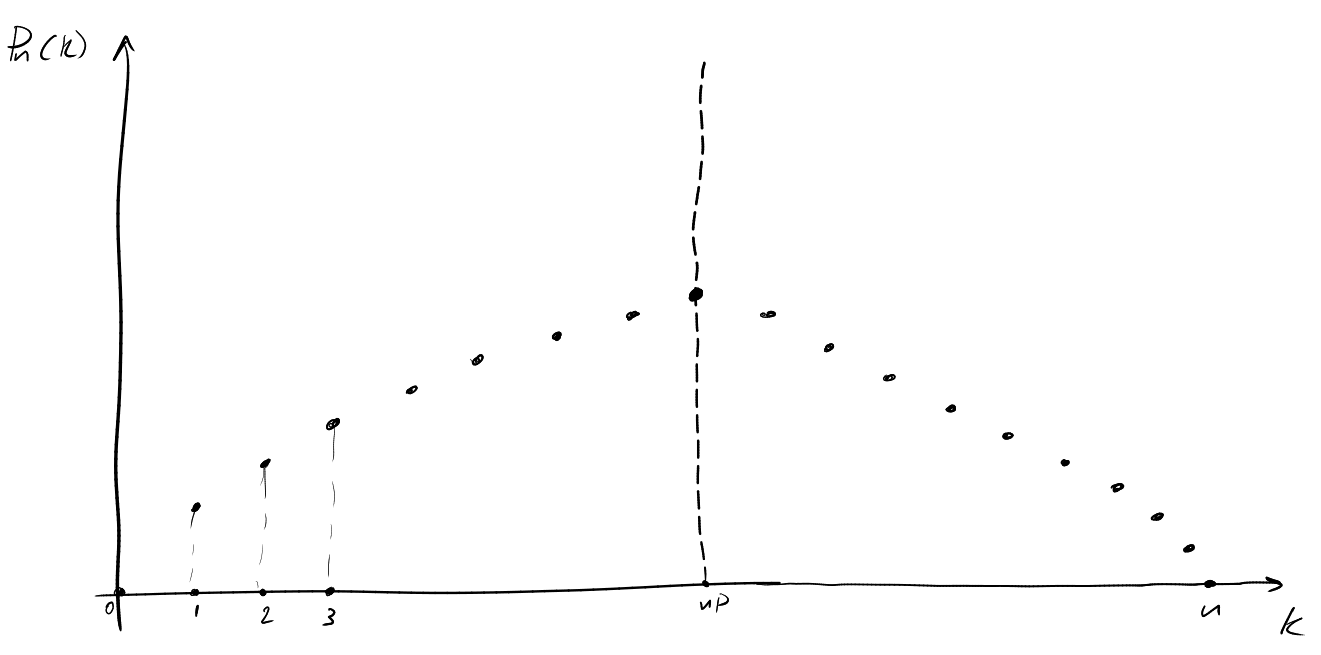
\includegraphics[scale=0.35]{4_1.png}
\end{center}
\subsection{Предельные теоремы в схеме Бернулли}
\label{sec:org8b8bea6}
\begin{definition}
\textbf{Локальная формула} Муавра-Лапласса. Применяем когда требуется найти вероятноть точного числа успехов.
\[ P_n(\nu_n = x) \approx \frac{1}{\sqrt{npq}}\varphi(x) \]
, где \(\varphi(x) = \frac{1}{\sqrt{2\pi}}e^{-\frac{x^2}{2}}, x = \frac{k - np}{\sqrt{npq}}\) --- функция Гауса. \\
Свойства функции Гауса \(\varphi(x)\):
\begin{enumerate}
\item \(\varphi(-x) = \varphi(x)\) --- четная
\item при \(x > 5,\ \varphi(x) \approx 0\)
\end{enumerate}
\end{definition}
\begin{definition}
\textbf{Интегральная формула Лапласса}. Применяем если число успехов лежит в неком диапозоне.
\[ P_n(x_1 \le \nu_n \le x_2) \approx \Phi(x_1) - \Phi(x_2) \]
, где \[ \Phi(x) = \frac{1}{\sqrt{2\pi}} \int_0^x e^{-\frac{z^2}{2}} dz\] --- функция Лапласса \\
\[ x_1 = \frac{k_1 - np}{\sqrt{npq}},\ x_2 = \frac{k_2 - np}{\sqrt{npq}} \]

Свойства \(\Phi(x)\):
\begin{enumerate}
\item \(\Phi(-x) = \Phi(x)\) --- нечетная
\item при \(x > 5,\ \Phi(x) \approx 0.5\)
\end{enumerate}
\end{definition}
\begin{remark}
В некоторых источниках под функцией Лапласса подразумевается несколько иная функция, чаще всего:
\[ F_0(x) = \frac{1}{\sqrt{2\pi}} \int_{-\infty}^x e^{z^2}{2}dz \]
\[ F_0(x) = 0.5 + \Phi(x)\text{ или }\Phi(x) = F_0(x)-0.5 \]
\end{remark}
\begin{remark}
Формулу применяем при \(n \ge 100\) и \(p,q\ge0.1\) 
\end{remark}
\begin{task}
Вероятность попадания стрелка в цель при одном выстреле 0.8. Стрелок сделал 400 выстрелов. Найти вероятность того что
\begin{enumerate}
\item произошло ровно 330 попаданий
\item произошло от 312 до 336 попаданий
\end{enumerate}
\end{task}
\begin{solution}
\-
\begin{enumerate}
\item \(n = 400, p = 0.8, q = 0.2, k=330\)
\[ x = \frac{330 - 400\cdot0.8}{\sqrt{400\cdot0.8\cdot0.2}} = 1.25 \]
\[ P_{400}(330) \approx \frac{1}{8} \cdot \varphi(1.25) \approx \frac{1}{8}\cdot0.1826 \approx 0.0228 \]
\item \(n = 400, p=0.8, q = 0.2, k_1 =312, k_2 = 336\)
\[ x_1 = \frac{312 - 400\cdot0.8}{\sqrt{400\cdot0.8\cdot0.2}} = -1\]
\[ x_2 = \frac{336 - 400\cdot0.8}{\sqrt{400\cdot0.8\cdot0.2}} = 2\]
\[ P_{400}(312 \le \nu_n \le 336) = \Phi(2) - \Phi(-1) = \Phi(2) + \Phi(1) \approx 0.8185 \]
\end{enumerate}
\end{solution}
\section{Статистическое определение вероятности}
\label{sec:org8f4f0f6}
\begin{itemize}
\item \(n_A\) --- число появления события \(A\) при \(n\) испытаниях
\item \(\frac{n_A}{n}\) --- частота события \(A\)
\end{itemize}
\[ P(A) \approx \frac{n_A}{n}, \text{при }n\to\infty \]

\subsection{Вероятность отклонения относительной частоты}
\label{sec:org88174c7}
\(] p\) --- веротяность события \(A\), \(\frac{n_A}{n}\) --- частота \(A\) \\
По интегральной формуле Лапласса:
\[ P\left(\left|\frac{n_A}{n} - p| \le \varepsilon\right) = P(-\varepsilon \le \frac{n_A}{n} - p \le \varepsilon) = P(-n\varepsilon \le n_a - np \le n\varepsilon) = P(np - n\varepsilon \le n_A \le np + n\varpepsilon) \]
\[ x_1 = \frac{np - n\varepsilon - np}{\sqrt{npq}} = -\frac{n\varepsilon}{\sqrt{npq}} \]
\[ x_2 = \frac{np + n\varepsilon - np}{\sqrt{npq}} = \frac{n\varespilon}{\sqrt{npq}} \]
\[ P\left(\left|\frac{n_A}{n} - p\right| \le \varepsilon\right) = \Phi\left(\frac{n\varepsilon}{\sqrt{npq}}\right) - \Phi\left(-\frac{n\varepsilon}{\sqrt{npq}}\right) = 2\Phi\left(\frac{n\varepsilon}{\sqrt{npq}}\right) \]
\[ P\left(\left|\frac{n_A}{n} - p\right| \le \varepsilon\right) = 2\Phi\left(\frac{\sqrt{n}}{\sqrt{pq}}\varepsilon\right) \]
\subsection{Закон больших чисел Бернулли}
\label{sec:org5c537f9}
Более точно последняя формула выглядит так:
\[ P\left(\left|\frac{n_A}{n} - p\right| \le \varepsilon\right) \xrightarrow[n \to \infty]{} 2\Phi\left(\frac{\sqrt{n}}{\sqrt{pq}}\varepsilon\right) \]
при \(n \to \infty\) \(\frac{\sqrt{n}}{\sqrt{pq}}\varepsilon \to \infty\) и \(\Phi\left(\frac{\sqrt{n}}{\sqrt{pq}}\right) \to 0.5\)
\[ P\left(\left|\frac{n_A}{n} - p\right| \le \varepsilon\right) \to 2\cdot0.5 = 1\]
\[ \lim_{n\to\infty}P\left(\left|\frac{n_A}{n} - p \right| \le \varepsilon \right) = 1 \]
--- закон больших чисел Бернулли \\
То есть при большом числе испытаний, будет близко к реальной вероятности
\end{document}
